\documentclass[11pt,twoside,a4paper]{article}
\usepackage[english]{babel} 
\usepackage{hyperref}
\usepackage[margin=4cm]{geometry}
\usepackage[style=apa,hyperref,doi,url,backend=biber]{biblatex}
\usepackage{csquotes}
\usepackage{graphicx}
\DeclareLanguageMapping{english}{english-apa}
\title{Emergent Architecture Design} 
\author{
	Paul Bakker, pbakker3, 4326091 \\
    Robin Borst, robinborst, 4291972 \\
    Matthijs de Groot, mawdegroot, 4171683 \\
    Julian Hols, jthols, 4247930\\
    Jan van Rosmalen, javanrosmalen, 4318609\\
}
\addbibresource{references.bib}

\begin{document}
\maketitle
\newpage
\tableofcontents
\newpage

\section{Introduction}

To implement our product we will have different design goals so we can satisfy the needs of the customer. These are described here below. In section 2 we will describe the software architecture views of our product.

\subsection{Design Goals}
\subsubsection{Usability}
The most important design goal that we have is usability. It is important that the user can execute the program really efficiently and in a rapid order. That is the reason that we want to make the program executable via the command line. This allows the user to script multiple calls to the program to get the data from multiple patients. Because the customer has indicated that he knows how the command line call works, we think this is the best implementation to execute the program. This enhances the usability for the analyst as he can process a lot of data really quickly.
\subsubsection{Modularity}
The modularity design goal means that we will define the individual components well, which leads to better maintenance. Also because we work with five people it is beneficial to have good modularity as we can each work on an individual component. And good modularity also helps us greatly in realizing our next design goal.
\subsubsection{Re-usability}
The re-usability design goal means that we will be able to reuse almost all of the code for other customers. We could for example reuse most of the code to easily get the same functionality for other self-monitoring projects.
\subsubsection{Compatibility}
The compatibility design goal means that the software is able to operate with different file formats outputted by other software products. We will use this to accept multiple file formats for the import and export. The exported files then can be used by different statistics analysis programs.
\newpage
\section{Software Architecture Views}
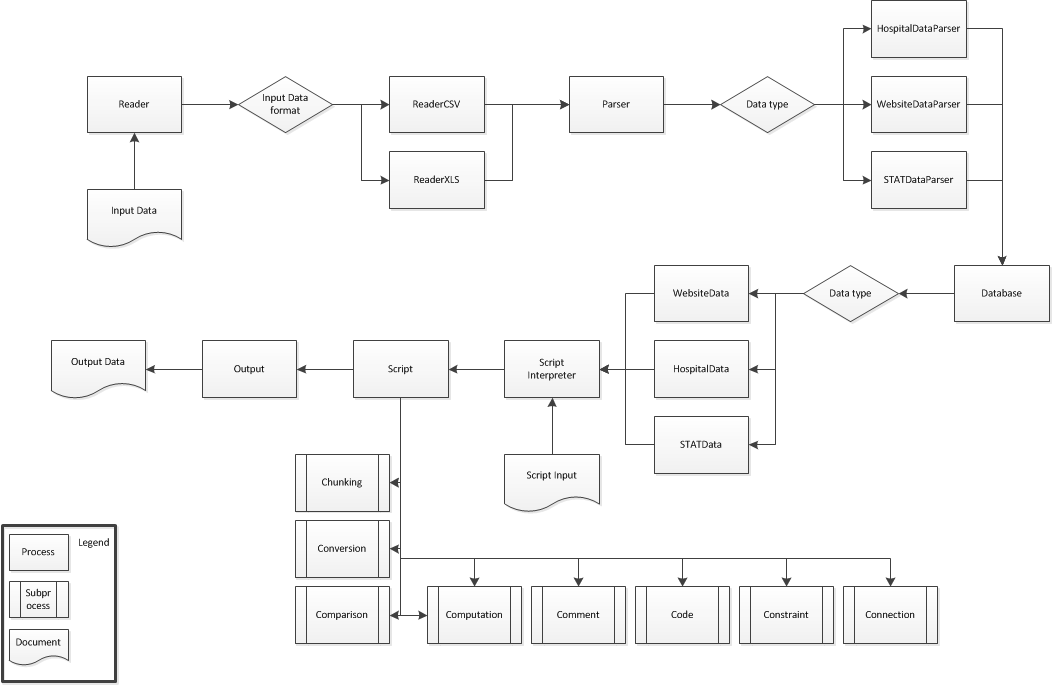
\includegraphics[scale=0.5]{FlowDiagram.png}


\subsection{Subsystem decomposition}
We will divide our product into different components, which we will describe below. 

\begin{itemize}
\item The main class:
\\	The main is the class that the customer will call using the command line. This will call the correct parser.
\item Parser interface: 
\\ The parser will read data line by line from the Reader interface and output this data into a correct data-structure.
\item Reader interface :
\\ The reader will read the data file and outputs it to an inputstream.
\item Database class:
\\ The subclasses of the database class will store all the data during the before and during the data processing.
\item ScriptInterpreter class:
\\ The ScriptInterpreter class will read the script file and execute all the corresponding sequential data operations. It will output a data-structure predefined by us.
\item Output class:
\\ The Output class will generate a text file from the output of the ScriptInterpeter class. The user will be able to select the delimiter.
\end{itemize}

\subsection{Data management} 
Each data processing operation in the script will take an input data-structure and outputs the same data-structure so it can be used as input for the next processing operation.


\end{document}